%\documentclass[english, times, mirror]{revdetua}
% use this if you're writing in portuguese:
\documentclass[portuguese, times, mirror]{revdetua}

\usepackage[utf8]{inputenc}
\usepackage{graphicx}
\usepackage{hyperref}

\usepackage{amsmath}
\usepackage{mathtools}

\usepackage{caption}
\usepackage{listings}
\usepackage{color}

\definecolor{dkgreen}{rgb}{0,0.6,0}
\definecolor{gray}{rgb}{0.5,0.5,0.5}
\definecolor{mauve}{rgb}{0.58,0,0.82}

\lstset{frame=tb,
  language=Java,    
  aboveskip=3mm,
  belowskip=3mm,
  showstringspaces=false,
  columns=flexible,
  basicstyle={\small\ttfamily},
  numbers=none,
  numberstyle=\tiny\color{gray},
  keywordstyle=\color{blue},
  commentstyle=\color{dkgreen},
  stringstyle=\color{mauve},
  breaklines=true,
  breakatwhitespace=true,
  tabsize=3
}

\usepackage{tikz}
\usepackage{pgfplots}

% correct bad hyphenation here
\hyphenation{op-tical net-works semi-conduc-tor}

\begin{document}

\Header{1}{5}{Outubro}{2016}{1}
% Note: the month must be in Portuguese

\title{Visão por Computador 2016-17, Guia Prático N.º 9}
\author{Rui Oliveira, Tomás Rodrigues\\ DETI, Universidade de Aveiro \\ Aveiro, Portugal \\ \{ruipedrooliveira, tomasrodrigues\}@ua.pt}
% you should be able to use the \and keyword, but the deti format doesn't like it, for some reason
\maketitle

\begin{resumo}


Pretende-se através deste relatório expor sob forma escrita, o nosso desempenho e objetivos alcançados na aula prática n.º9 da unidade curricular de Visão por Computador do Mestrado Integrado de Engenharia de Computadores e Telemática.

Neste relatório pretenderemos explicar as soluções por nós encontradas para a resolução dos diferentes problemas propostos.


\end{resumo} 

\begin{palavraschave} %
visão, computador, imagem digital, tracking, movement, background, foreground, opencv, c++, 
 \end{palavraschave} %


\section{Repositório: código fonte}


Todas as soluções dos problemas propostos estão disponível através do seguinte repositório (gitHub) criado para o efeito. \\

\href{http://github.com/toomyy94/CV1617-68779-68129}{http://github.com/toomyy94/CV1617-68779-68129}
\\


A resolução dos problemas do presente guia encontram-se na pasta aula9. Para a resolução dos exercícios não foi usado nenhum IDE. Para a compilação do código fonte foi usada uma makefile. 



\section{Problemas propostos}



\subsection{Problema \#1 - \textit{Optical flow}}

\subsubsection{Enunciado}
\textit{Explore the OpenCV example of Lucas-Kanade optical flow algorithm. Adapt the referred exam-
ple to detect moving objects in a static scene, considering also that the camera is fixed.}


\subsubsection{Resolução e principais conclusões}

Para a resolução deste exercício foram seguidos os seguintes passos: 

\begin{itemize}
    \item Primeiro as capturas dos frames do vídeo
    \item Passagem do frame para GRAY com a função \textit{cvtColor} utilizada em guiões passados
    \item O cálculo do optical flow é feito com a função \textit{calcOpticalFlowFarneback} e posteriormente são desenahdas linhas na direção do movimento, similarmente ao exemplo apresenado na aula.
    \item Finalmente o desenho das linhas e a visualização da imagem pós processamento.
\end{itemize}

\begin{lstlisting}[caption=Excerto do código de processamento,label=code:C]
for (int y = 0; y < original.rows; y += 5) {
+         for (int x = 0; x < original.cols; x += 5)
+         {
+                  // get the flow from y, x position * 10 for better visibility
+            const Point2f flowatxy = flow.at<Point2f>(y, x) * 10;
+                         // draw line at flow direction
+            line(original, Point(x, y), Point(cvRound(x + flowatxy.x), cvRound(y + flowatxy.y)), Scalar(0,0,255));
+                                                             // draw initial point
+            circle(original, Point(x, y), 1, Scalar(0, 0, 0), -1);
+          }
+
+         }
\end{lstlisting}

O resultado obtidos pode ser observado na seguinte figura. 

\begin{figure}[ht!]
\centering
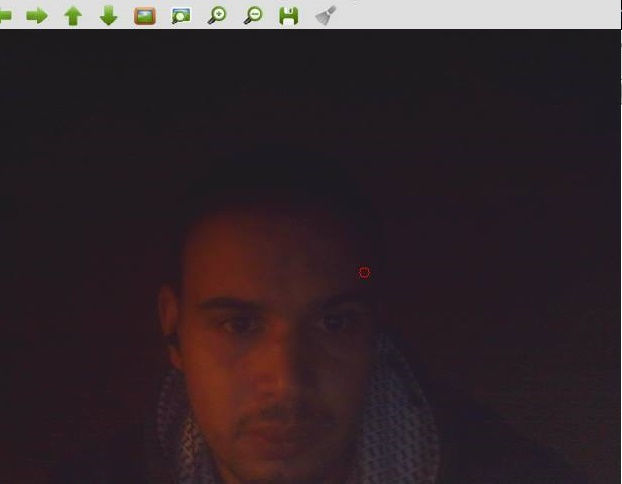
\includegraphics[width=70mm]{img/ex1.jpg}
\caption{Resultado obtido após exercício 1}
\end{figure}


%%%%%%%%%%%%%%%%%%%%%%%%%%%%%%%%%%%%%%%%%%%%%%%%%%%%%%%%%%%%%%5
%%%%%%%%%%%%%%%%%%%%%%%%%%%%%%%%%%%%%%%%%%%%%%%%%%%%%%%%%%%%%%%

\subsection{Problema \#2 - \textit{Fore/Background separation}}

\subsubsection{Enunciado}
\textit{Implement a program to capture video from your digital camera or or load a video file and develop
an algorithm to perform background/foreground separation. Start by a supervised solution where
the user can specify what is the background frame.}


\subsubsection{Resolução e principais conclusões}

A implementação deste exercício não foi conseguida devido à nossa versão do opencv ser inferior à 3.1.0. Os tuturiais e implementações que encontrámos para retirar o background em tempo real através da camâra usam 
\begin{lstlisting}[caption=Aplicação da função createBackgroundSubtractorMOG2 ,label=code:C]
pMOG2 = createBackgroundSubtractorMOG2(); //MOG2 approach
\end{lstlisting}

ou variantes, e que não existem nesta versão do opencv. No entanto testamos este código no opencv 3.1.0 e funcionava perfeitamente similiar ao exemplo que o professor demonstrou na aula.

%%%%%%%%%%%%%%%%%%%%%%%%%%%%%%%%%%%%%%%%%%%%%%%%%%%%%%%%%%%%%%5
%%%%%%%%%%%%%%%%%%%%%%%%%%%%%%%%%%%%%%%%%%%%%%%%%%%%%%%%%%%%%%%


\subsection{Problema \#3 - \textit{Object Tracking}}


\subsubsection{Enunciado}
\textit{Implement a program to capture video from your digital camera or or load a video file and explore
the OpenCV algorithms to perform object tracking. }

\subsubsection{Resolução e principais conclusões}

Para a resolução deste exercício foram seguidos os seguintes passos: 

Primeiramente ligámos a câmera para uma captura de frames em tempo real. Depois ao clicar na imagem é adicionado um ponto, se o algoritmo encontrar um ponto bom/viável para prosseguir com o track.

Apartir daí o(s) ponto(s) adicionados são seguidos à medida que o foreground se movimenta. Se os pontos sairem do plano da camâra são imediatamente removidos e o tracking perde-se.


\begin{lstlisting}[caption=Excerto de código,label=code:C]
if( needToInit )
        {
            // automatic initialization
            goodFeaturesToTrack(gray, points[1], MAX_COUNT, 0.01, 10, Mat(), 3, 0, 0.04);
            cornerSubPix(gray, points[1], subPixWinSize, Size(-1,-1), termcrit);
            addRemovePt = false;
        }
        else if( !points[0].empty() )
        {
            vector<uchar> status;
            vector<float> err;
            if(prevGray.empty())
                gray.copyTo(prevGray);
            calcOpticalFlowPyrLK(prevGray, gray, points[0], points[1], status, err, winSize,
                                 3, termcrit, 0, 0.001);
            size_t i, k;
            for( i = k = 0; i < points[1].size(); i++ )
            {
                if( addRemovePt )
                {
                    if( norm(point - points[1][i]) <= 5 )
                    {
                        addRemovePt = false;
                        continue;
                    }
                }

                if( !status[i] )
                    continue;

                points[1][k++] = points[1][i];
                circle( image, points[1][i], 3, Scalar(0,255,0), -1, 8);
            }
            points[1].resize(k);
        }
\end{lstlisting}

O resultado obtidos pode ser observado na seguinte figura:

\begin{figure}[ht!]
\centering
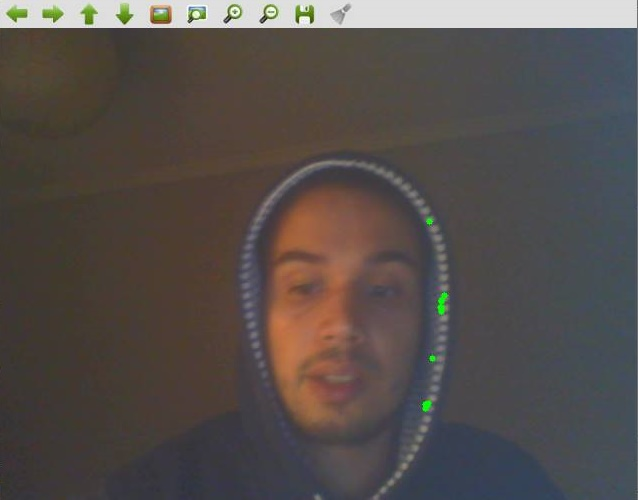
\includegraphics[width=70mm]{img/ex3.jpg}
\caption{Resultado obtido após exercício 3}
\end{figure}



%%%%%%%%%%%%%%%%%%%%%%%%%%%%%%%%%%%%%%%%%%%%%%%%%%%%%%%%%%%%%%5
%%%%%%%%%%%%%%%%%%%%%%%%%%%%%%%%%%%%%%%%%%%%%%%%%%%%%%%%%%%%%%%


\begin{thebibliography}{1} % 9

\bibitem{fsound}
Neves, A. J. R.; Dias, P. Slides teóricos Visão por Computador - Aula 9 (2016)

\bibitem{vtk}
OpenCV. \href{hhttp://docs.opencv.org/}{Opencv Documentation}. Web. 15 Outubro 2016. 




\end{thebibliography}

\end{document}
